\chapter{Diseño e Implementación} % Main chapter title

\label{Chapter3} % Change X to a consecutive number; for referencing this chapter elsewhere, use \ref{ChapterX}

\definecolor{mygreen}{rgb}{0,0.6,0}
\definecolor{mygray}{rgb}{0.5,0.5,0.5}
\definecolor{mymauve}{rgb}{0.58,0,0.82}

%%%%%%%%%%%%%%%%%%%%%%%%%%%%%%%%%%%%%%%%%%%%%%%%%%%%%%%%%%%%%%%%%%%%%%%%%%%%%
% parámetros para configurar el formato del código en los entornos lstlisting
%%%%%%%%%%%%%%%%%%%%%%%%%%%%%%%%%%%%%%%%%%%%%%%%%%%%%%%%%%%%%%%%%%%%%%%%%%%%%
\lstset{ %
  backgroundcolor=\color{white},   % choose the background color; you must add \usepackage{color} or \usepackage{xcolor}
  basicstyle=\footnotesize,        % the size of the fonts that are used for the code
  breakatwhitespace=false,         % sets if automatic breaks should only happen at whitespace
  breaklines=true,                 % sets automatic line breaking
  captionpos=b,                    % sets the caption-position to bottom
  commentstyle=\color{mygreen},    % comment style
  deletekeywords={...},            % if you want to delete keywords from the given language
  %escapeinside={\%*}{*)},          % if you want to add LaTeX within your code
  %extendedchars=true,              % lets you use non-ASCII characters; for 8-bits encodings only, does not work with UTF-8
  %frame=single,	                % adds a frame around the code
  keepspaces=true,                 % keeps spaces in text, useful for keeping indentation of code (possibly needs columns=flexible)
  keywordstyle=\color{blue},       % keyword style
  language=[ANSI]C,                % the language of the code
  %otherkeywords={*,...},           % if you want to add more keywords to the set
  numbers=left,                    % where to put the line-numbers; possible values are (none, left, right)
  numbersep=5pt,                   % how far the line-numbers are from the code
  numberstyle=\tiny\color{mygray}, % the style that is used for the line-numbers
  rulecolor=\color{black},         % if not set, the frame-color may be changed on line-breaks within not-black text (e.g. comments (green here))
  showspaces=false,                % show spaces everywhere adding particular underscores; it overrides 'showstringspaces'
  showstringspaces=false,          % underline spaces within strings only
  showtabs=false,                  % show tabs within strings adding particular underscores
  stepnumber=1,                    % the step between two line-numbers. If it's 1, each line will be numbered
  stringstyle=\color{mymauve},     % string literal style
  tabsize=2,	                   % sets default tabsize to 2 spaces
  title=\lstname,                  % show the filename of files included with \lstinputlisting; also try caption instead of title
  morecomment=[s]{/*}{*/}
}


%----------------------------------------------------------------------------------------

En este capítulo se explica...

%----------------------------------------------------------------------------------------

\section{Prototipo de pruebas}

El prototipo de pruebas, fue desarrollado con la finalidad de probar todas las funciones de firmware que componen el trabajo y brindar una primera aproximación al prototipo comercial del dispositivo.

Como se vio en la figura 2.1, el dispositivo está compuesto por los siguientes bloques funcionales: microcontrolador, transceptor Wi-Fi, transceptor LoRa, memoria no volátil, reloj en tiempo real y conversor óptico-eléctrico.

La construcción del prototipo de pruebas se realizó en una \textit{breadboard}, para poder realizar cambios en las conexiones de los componentes de una manera sencilla cuando estos se requieran. Se eligieron componentes de hardware acordes con los bloques que constituyen el dispositivo, en su mayor parte módulos de desarrollo con circuitos integrados embebidos que disponen de conectores apropiados para una breadboard. En la figura 3.1 se muestra el diagrama en bloques general con los componentes del prototipo de pruebas.


\begin{figure}[h]
	\centering
	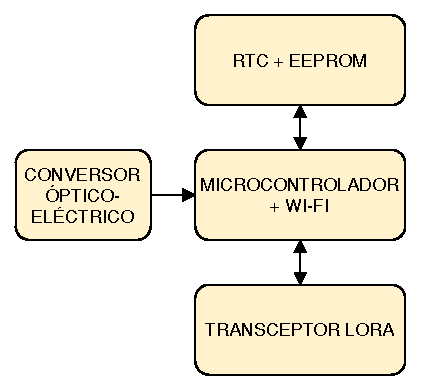
\includegraphics[scale=1]{./Figures/test_blocks.pdf}
	\caption{Diagrama en bloques del prototipo de pruebas.}
	\label{fig:blocksTest}
\end{figure}

Para garantizar un tiempo corto en la obtención de los componentes del prototipo de pruebas, el criterio predominante para la elección de los componentes de cada uno de los bloques fue la disponibilidad en el mercado local. Además, la elección de proveedores locales aseguró la restitución eficaz de los componentes que se malograron durante el desarrollo.

\subsection{Microcontrolador + Wi-Fi}

Este bloque fusiona los bloques microcontrolador y transceptor Wi-Fi. El desarrollo de dispositivos con conexión Wi-Fi ha tenido un gran crecimiento en los últimos años (ref), por lo que los fabricantes de circuitos integrados ofrecen soluciones que integran microcontroladores y transceptores Wi-Fi en un solo encapsulado.

El componente elegido para este bloque es la tarjeta de desarrollo NodeMCU de la firma Amica, basado en el módulo ESP-12F de la firma Ai-Thinker. Las características más atractivas de esta tarjeta en lo referente al desarrollo, son alimentación y programación a través de un puerto micro USB, factor de forma adecuado para ser montado sobre un breadboard e incorporación de LEDs y pulsadores en la misma tarjeta. En la figura 3.2 se muestra la NodeMCU.

\begin{figure}[h]
	\centering
	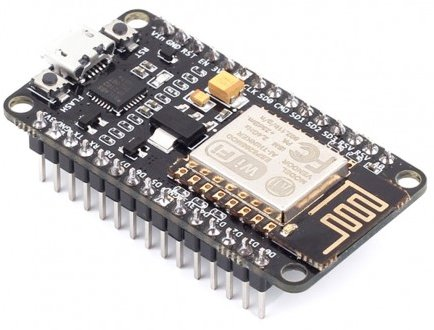
\includegraphics[scale=0.5]{./Figures/nodemcu.jpg}
	\caption{Tarjeta de desarrollo NodeMCU de la firma Amica\protect\footnotemark.}
		\label{fig:cuadradoAzul}
	\end{figure}

	\footnotetext{Imagen tomada de: \url{https://www.amazon.com/-/es/KeeYees-Internet-Development-Wireless-Compatible/dp/B07PR9T5R5}}

El módulo ESP-12F, monta sobre sí un SoC (\textit{System on a Chip}, sistema en un chip) de la firma Espressif Systems, el ESP8266, que funciona como microcontrolador y transceptor Wi.Fi. Otros componentes instalados sobre este módulo son condensadores, resistencias, oscilador, memoria flash y una antena impresa; todos ellos necesarios para que el ESP8266 pueda desempeñar correctamente sus funciones.

El ESP8266 es un chip de bajo costo que incorpora un microcontrolador y un transceptor Wi-Fi, además de contar con un \textit{stack} TCP/IP. Sus características técnicas más relevantes son:
\begin{itemize}
	\item Procesador: Tensilica LX106 de arquitectura RISC(footnote) de 32 bits a una frecuencia de 80 MHz.
	\item RAM: 64 KB para instrucciones y 96 KB para datos.
	\item ROM: externa, puede soportar hasta 16 MB de memoria flash con conexión QSPI(footnote).
	\item Wi-Fi: IEEE 802.11 b/g/n.
	\item Periféricos: GPIO, SPI, I\textsuperscript{2}C, UART y ADC.
\end{itemize}

\subsection{Transceptor LoRa}

La elección del componente de este bloque, 

\subsection{RTC + EEPROM}

Los bloques memoria no volátil y reloj en tiempo real fueron fusionados en un único bloque, ya que comercialmente existen módulos que cumplen ambas funciones. Estos módulos tienen embebidos circuitos integrados de memoria y RTC, además de otros componentes como resistencias, condensadores, osciladores, zócalos para baterías y conectores apropiados para un breadboard. Estos módulos en su gran mayoría poseen una EEPROM como medio de almacenamiento de datos, esta tecnología es preferible sobre las memorias flash en aplicaciones de adquisición de datos, ya que proporciona un número mayor de ciclos de escritura y borrado.

La mayor parte de los módulos que existen en el mercado local cumplen cabalmente con las funciones que requiere este bloque, pero, debido a la cantidad de pines utilizables de la NodeMCU se tuvo preferencia por los módulos que tenían integrados chips con interfaz I\textsuperscript{2}C. Asimismo, al haber muchos módulos que cumplían el requisito de la interfaz, se buscó uno que tuviera un RTC con la capacidad de generar alarmas en función de la hora. En la figura 3.2 se observa el módulo de RTC + EEPROM elegido.

\begin{figure}[h]
	\centering
	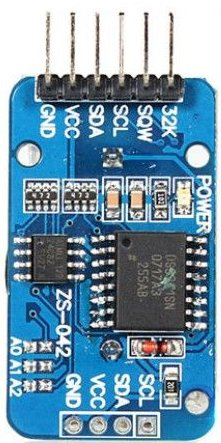
\includegraphics[scale=0.45]{./Figures/rtc_eeprom.jpg}
	\caption{Módulo RTC + EEPROM\protect\footnotemark.}
		\label{fig:cuadradoAzul}
	\end{figure}

	\footnotetext{Imagen tomada de: \url{https://electropeak.com/extremely-accurate-rtc-module}}

Los circuitos integrados que componen el módulo son el DS3231 y el AT24C32, un RTC y una EEPROM, respectivamente. El DS3231 es un RTC de alta precisión de la firma Maxim Integrated, que cuenta con una interfaz I\textsuperscript{2}C para conectarse con otros dispositivos, también tiene la capacidad de generar alarmas y medir la temperatura. El AT24C32 es una EEPROM de la firma Microchip, con interfaz I\textsuperscript{2}C y 32KB de capacidad de almacenamiento.

\subsection{Conversor óptico-eléctrico}

Para este bloque, el componente elegido es un módulo detector de luz, compuesto por un fototransistor PT333-3C de la firma Everlight y un comparador de voltaje LM393 de la firma Texas Instruments. El módulo genera como salida un pulso eléctrico acotado al nivel de voltaje con el que se alimenta, que está determinado por la cantidad de luz incidente y el valor del potenciómetro incluido. En la figura 3.3 se puede observar el módulo.

\begin{figure}[h]
	\centering
	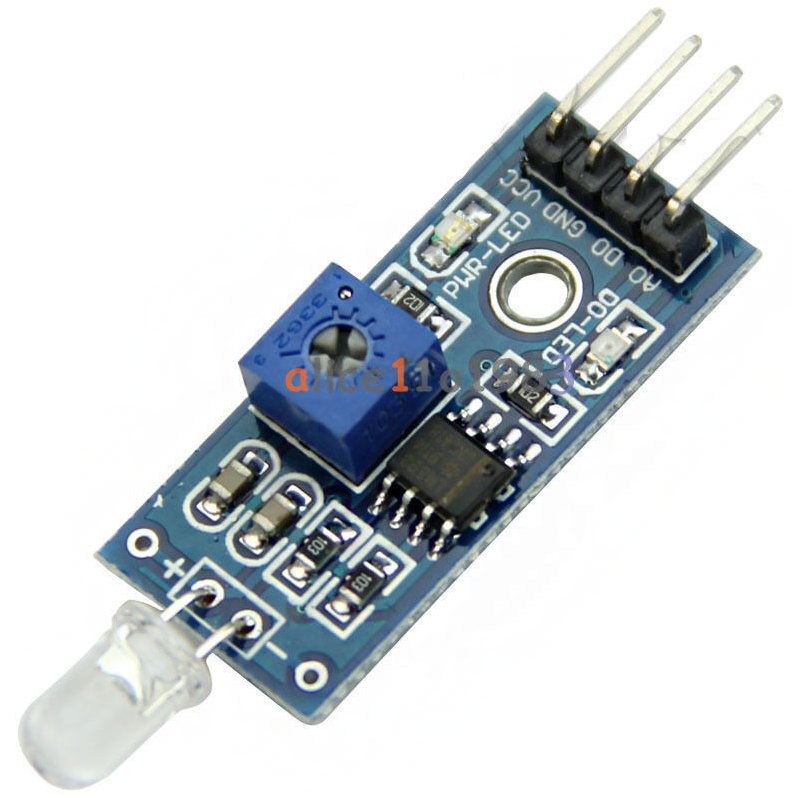
\includegraphics[scale=0.2]{./Figures/coe.jpg}
	\caption{Módulo detector de luz\protect\footnotemark.}
		\label{fig:cuadradoAzul}
\end{figure}

	\footnotetext{Imagen tomada de: \url{https://www.roboter-bausatz.de/en/diy-electronics/extension-modules/sensors/optics-light/149/light-sensor-module}}

%----------------------------------------------------------------------------------------

\section{Diseño de firmware}



%----------------------------------------------------------------------------------------

\section{Interfaz web}

%----------------------------------------------------------------------------------------

\section{Prototipo comercial}

El desarrollo de un prototipo para ser comercializado, fue necesario para una primera implementación del dispositivo en un entorno real de trabajo y la realización de pruebas a nivel físico. El mismo consta de una carcasa y un PCB (\textit{Printed Circuit Board}, tarjeta de circuito impreso).

\subsection{Carcasa}

El primer paso, fue elegir una carcasa de dimensiones adecuadas, para que pueda ser montada directamente sobre un medidor de consumo eléctrico domiciliario. Para este fin, se estudió la posibilidad de diseñar una carcasa personalizada, pero, debido a los altos costos de producción a nivel de prototipo, esta idea fue rápidamente descartada. Entonces, después de realizar un análisis de las dimensiones de los medidores utilizados por COPELECT, se eligió una carcasa disponible en el mercado internacional, la VG-S43 de la firma Vange. La elección de esta carcasa sobre otras similares, fue debido a los zócalos que tenía, que se adecuaban perfectamente para que el fototransistor estuviera descubierto y tuviera vista directa con el LED del medidor eléctrico. En la figura x se puede apreciar el carcasa elegida.

\begin{figure}[h]
	\centering
	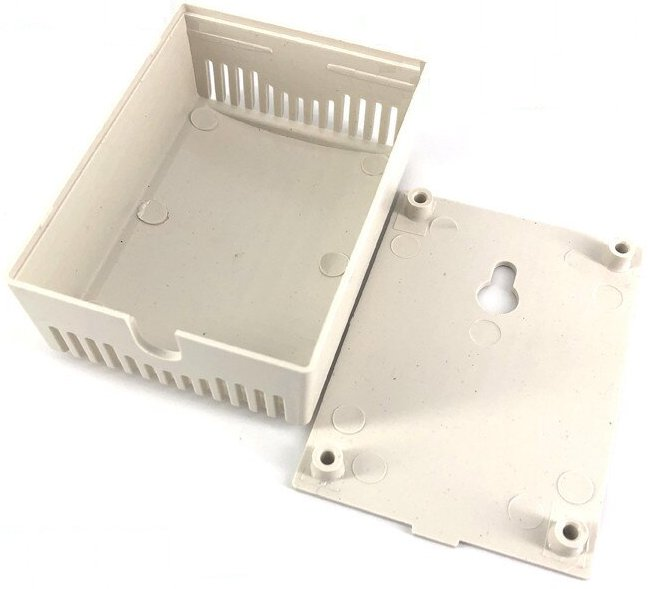
\includegraphics[scale=0.5]{./Figures/case.jpg}
	\caption{Carcasa VG-S43 de la firma Vange\protect\footnotemark.}
		\label{fig:cuadradoAzul}
\end{figure}

	\footnotetext{Imagen tomada de: \url{https://es.aliexpress.com/item/33004284623.html?spm=a2g0o.cart.0.0.50483c00xuS0Xo&mp=1}}

\subsection{Circuito impreso}

Antes de empezar con el diseño del PCB, se realizó la elección de los componentes que serían parte del mismo. En el prototipo de pruebas se utilizaron módulos y tarjetas de desarrollo que con el firmware implementado en ellos, cumplieron todos los requerimientos planteados. Entonces, para que el firmware desarrollado pudiera ser utilizado exitosamente en el prototipo comercial, se utilizaron los circuitos integrados principales de los módulos y tarjetas de desarrollo, también se descartaron los componentes electrónicos que no resultaban necesarios para este trabajo. Existen dos componentes que se implementaron como módulos, el ESP-12F que es componente principal de la NodeMCU, y el RA-01, que es un transceptor LoRa basado en el mismo circuito integrado que el PM1280, el SX1278. Además, el PT333-3C fue sustituido por el PT11-21C, que también es un fototransistor de similares características, pero es un SMD (\textit{Surface-Mount-Device}, dispositivo de montaje superficial).

Una vez elegidos los componentes implicados, se realizó un análisis del consumo de corriente de cada uno de ellos, para implementar una fuente de alimentación adecuada. Cabe resaltar que el voltaje de alimentación de de todos los componentes es 3,3 V. En la tabla x se muestran los valores máximos de consumo de corriente de los componentes, estos datos fueron obtenidos de los \textit{datasheets} de los mismos.

\begin{table}[h]
	\centering
	\caption[Consumo del prototipo comercial]{Tabla de consumo eléctrico de los componentes del prototipo comercial}
	\begin{tabular}{l c}    
		\toprule
		\textbf{Componente} & \textbf{Consumo de corriente (mA)} \\
		\midrule
		ESP-12F 	& 500 (en modo de transmisión continua) \\		
		RA-01		& 93 (en modo transmisor)\\
		DS3231		& 0,2 (en modo activo) \\
		AT24C32 	& 3 (cuando se escribe un dato)\\
		LM393 		& 20 (cortocircuitado a tierra) \\
		PT11-21C	& 20 \\
		\bottomrule
		\hline
	\end{tabular}
	\label{tab:componentsPower}
\end{table}

De la tabla anterior, se determinó que el consumo total de todos los componentes es de 636,2 mA. Al momento de elegir la fuente de alimentación al consumo total se le añadió un margen de seguridad del 50\%, dando un nuevo valor de 954,43 mA. Por lo tanto, la fuente de alimentación elegida debió ser de 3.3 V y 1 A.

Para reducir la cantidad de componentes de la fuente de alimentación, se escogió un módulo conversor de energía alterna a directa. De esta forma, el prototipo comercial podría conectarse directamente a la misma línea eléctrica del medidor. El componente elegido fue el módulo HLK-PM03 de la firma Hi-Link, que proporciona 3,3 V y 1 A a su salida, cuando a la entrada existen 90 V - 240 V alternos. En la figura x puede observarse el módulo para la fuente de alimentación.

\begin{figure}[h]
	\centering
	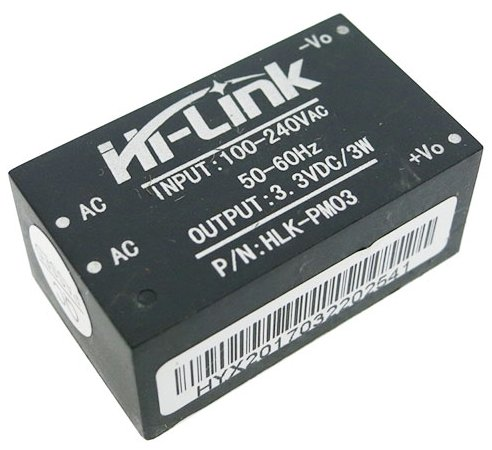
\includegraphics[scale=0.3]{./Figures/acdc_module.jpg}
	\caption{Módulo de alimentación HLK-PM03 de la firma Hi-Link.}
	\label{fig:blocksTest}
\end{figure}

Con ayuda del software KiCAD, se realizó el dibujo de un diagrama esquemático del prototipo comercial, que interconecta todos los componentes y brinda información relacionada a aspectos importantes sobre el funcionamiento y diseño del PCB. En la figura x se muestra el diagrama esquemático del prototipo comercial.

\begin{figure}[h]
	\centering
	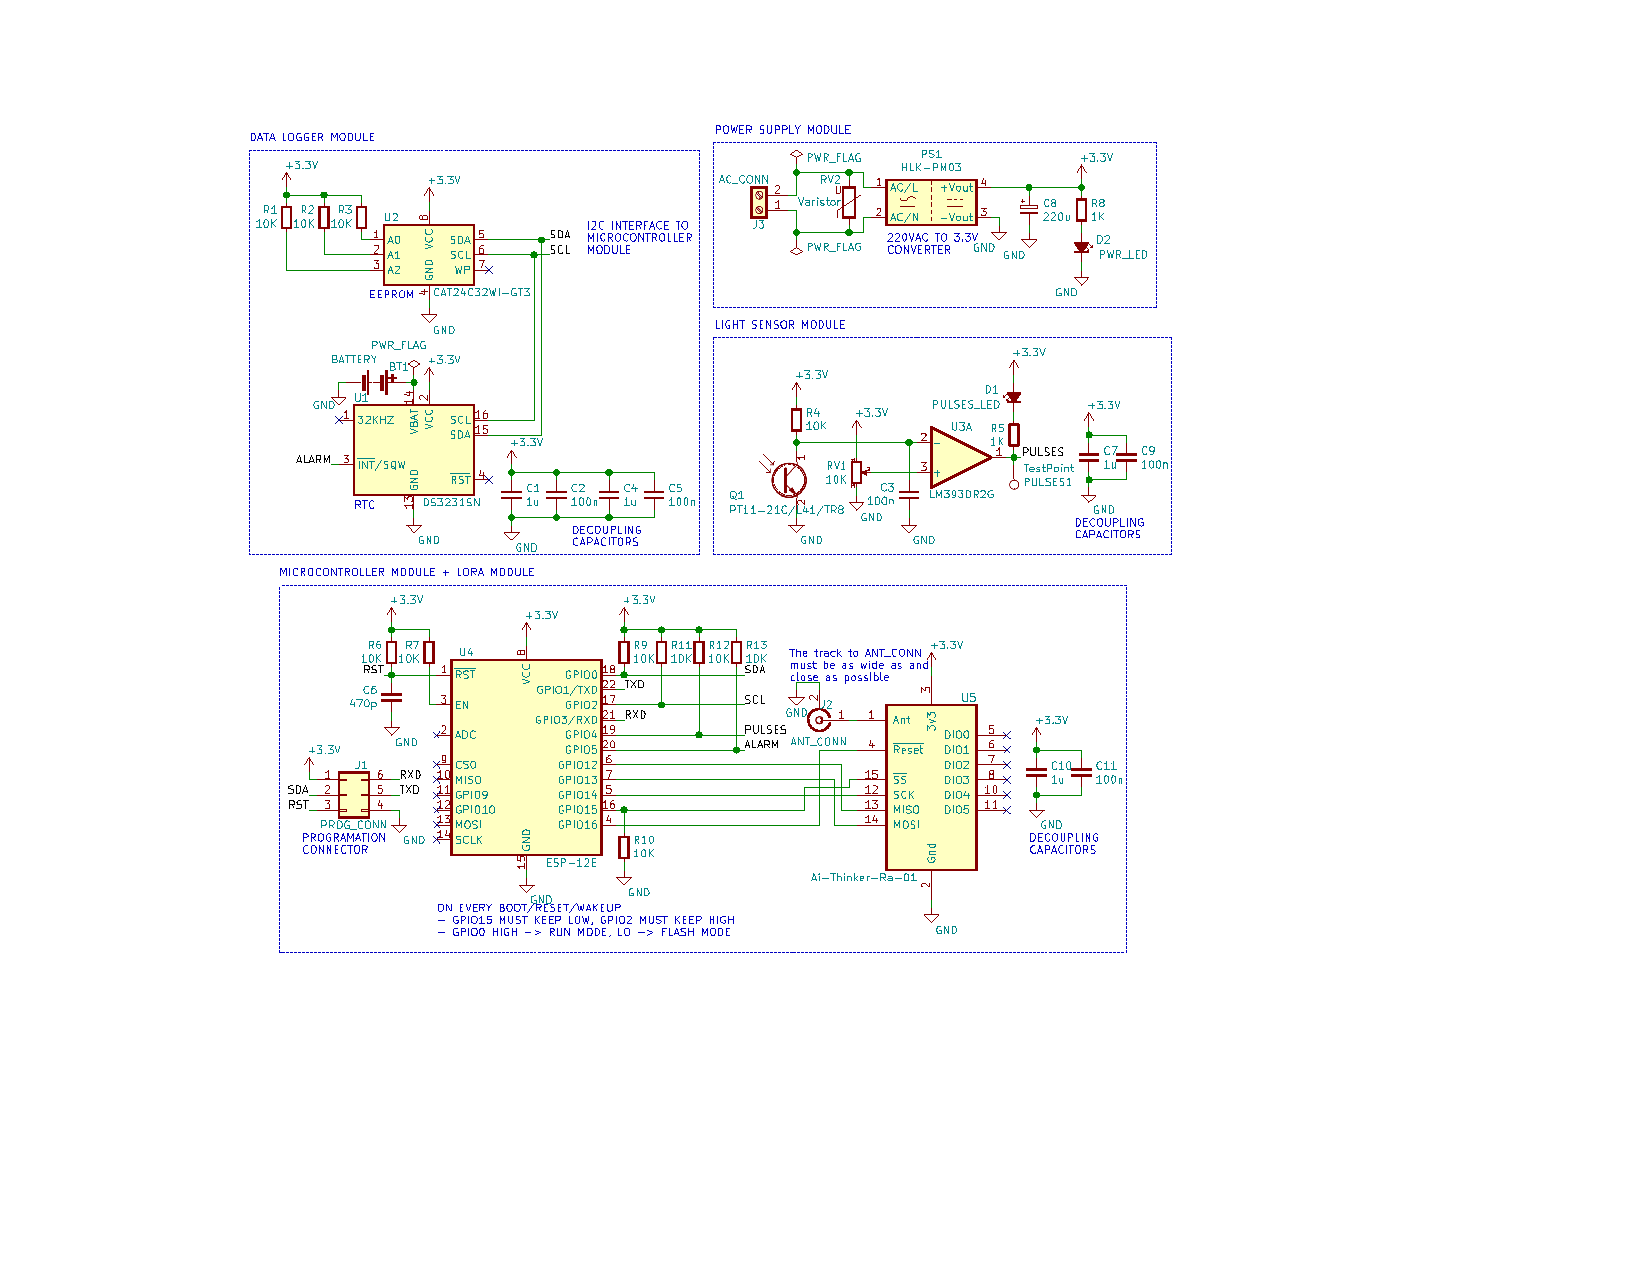
\includegraphics[scale=0.9]{./Figures/schematic.pdf}
	\caption{Diagrama esquemático del prototipo comercial.}
		\label{fig:cuadradoAzul}
\end{figure}

Del diagrama anterior, se puede notar que se añadieron \textit{test points} para poder probar la respuesta del sensor de luz mediante instrumentación especializada. Se añadieron también, un conector destinado a la depuración del código almacenado en el ESP8266, junto con LEDs para monitorear el estado de la fuente y el sensor de luz.

Con el diagrama esquemático finalizado, se realizó la ERC (\textit{Electrical Rule Check}, comprobación de reglas eléctricas) en busca posibles cortocircuitos, conexiones ilegales y contactos flotantes entre otras comprobaciones. Posteriormente, se dibujó el circuito impreso, donde se tuvieron en consideración las restricciones físicas impuestas por la elección de la carcasa. Se tuvo especial énfasis en la ubicación de los conectores, para que estos quedaran al borde del PCB y pudieran ser accedidos con mayor facilidad. El fototransistor quedó ubicado en una posición tal que coincidiera con el zócalo inferior de la carcasa. Otra consideración de importancia fue la distancia entre el transceptor LoRa y el conector coaxial, ambos componentes fueron ubicados muy cerca, de tal forma que la pista que los conectaba tuviera una distancia muy corta, asimismo, se dibujo la pista lo más ancha posible y se pusieron vías conectadas a tierra para lograr una mejor respuesta a las interferencias electromagnéticas.

Las capas \textit{top} y \textit{bottom} del PCB, pueden apreciarse en las figuras x y y, respectivamente. Por otro parte, en las figuras z y a, se muestran el modelo 3D renderizado del PCB y una fotografía del PCB montado.

\begin{figure}[h]
	\centering
	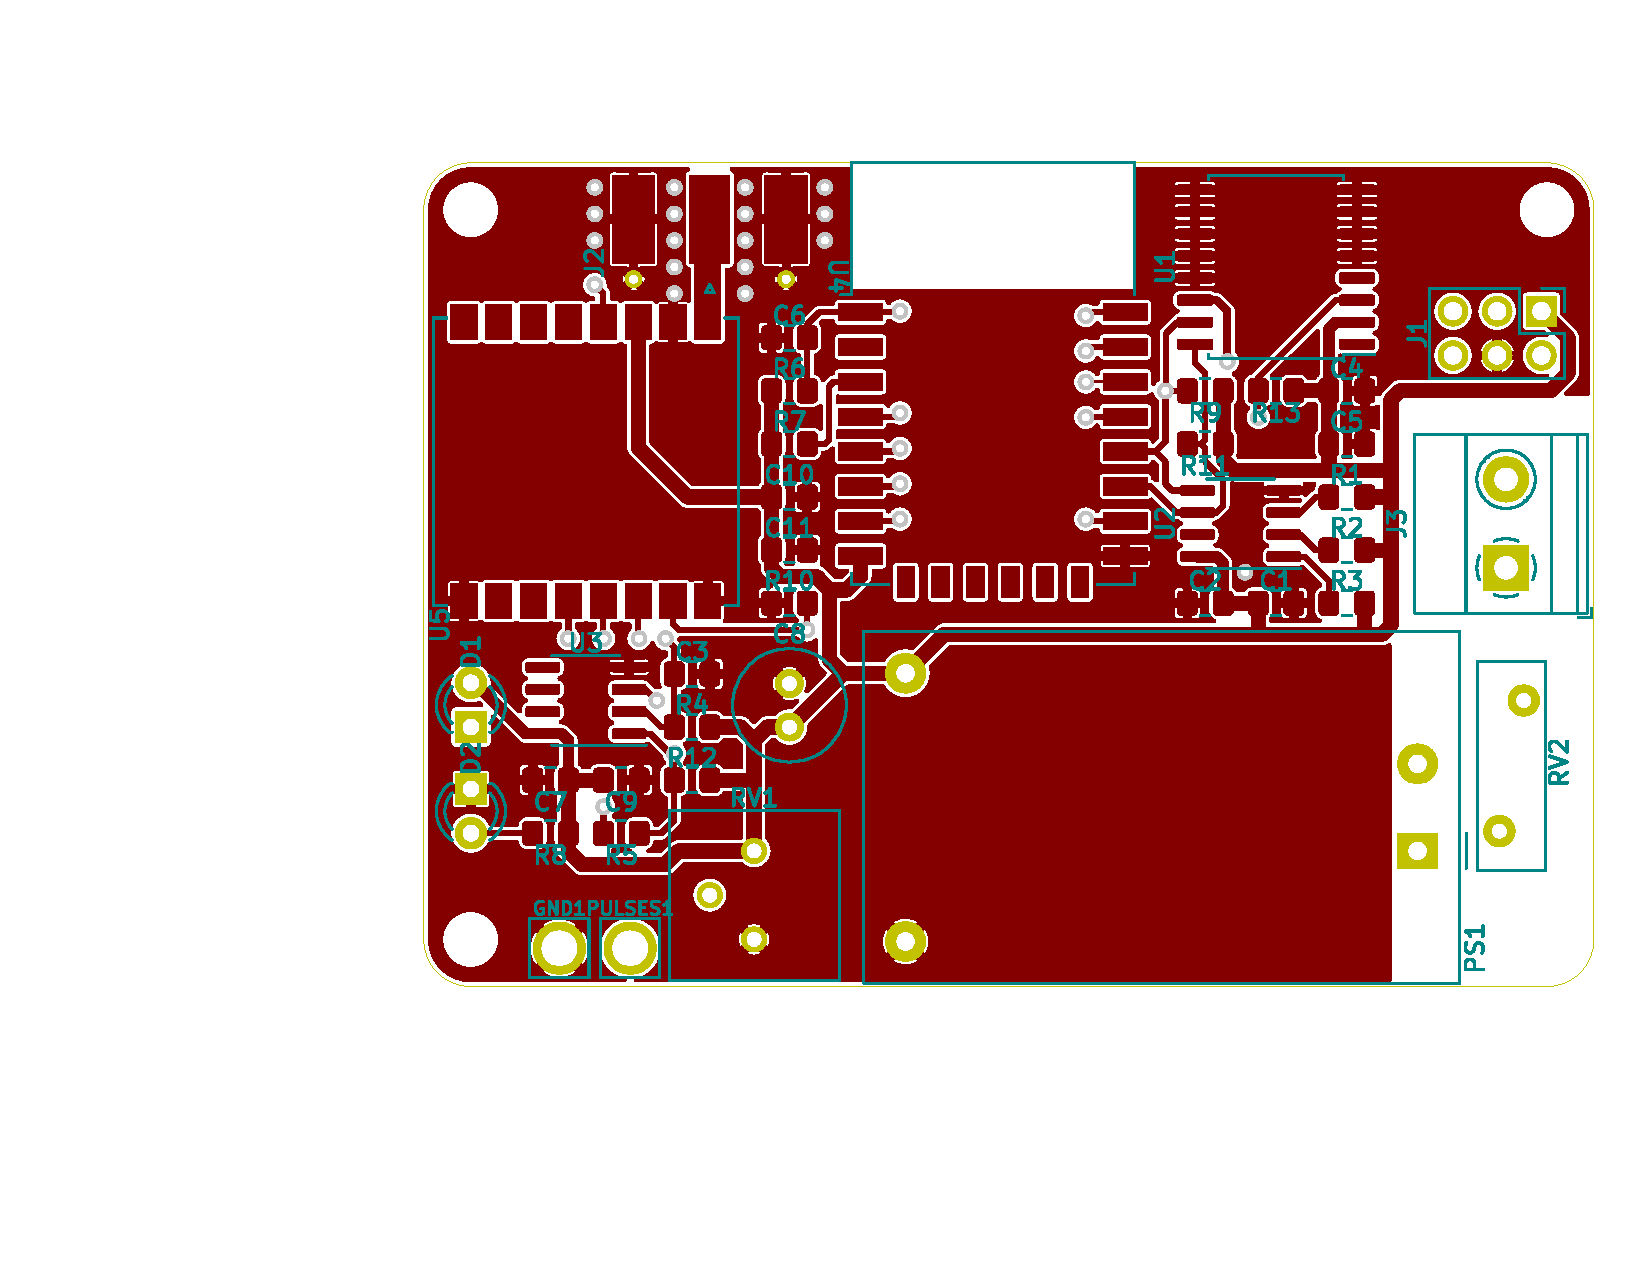
\includegraphics[scale=0.6]{./Figures/pcb_top.pdf}
	\caption{Capa top del PCB.}
		\label{fig:cuadradoAzul}
\end{figure}

\begin{figure}[h]
	\centering
	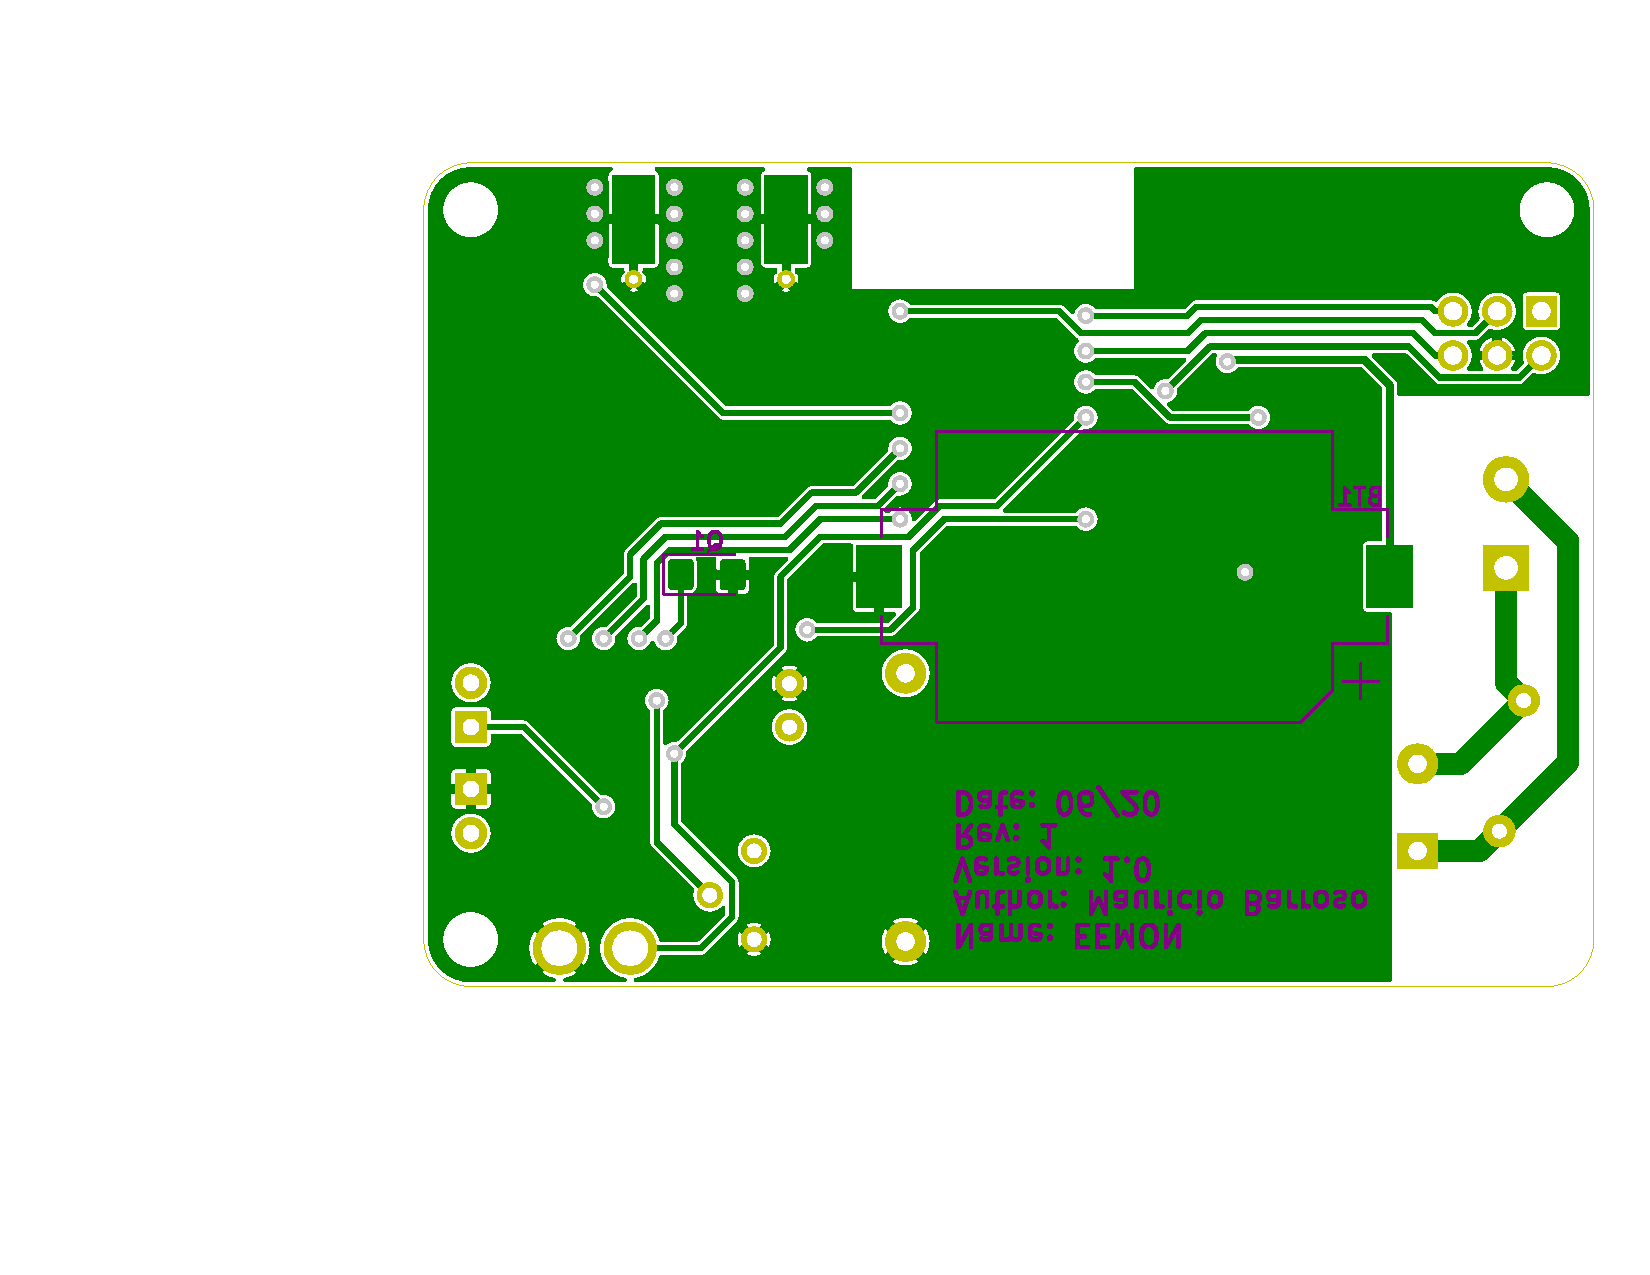
\includegraphics[scale=0.6]{./Figures/pcb_bot.pdf}
	\caption{Capa bottom del PCB.}
		\label{fig:cuadradoAzul}
\end{figure}

\begin{figure}[h]
	\centering
	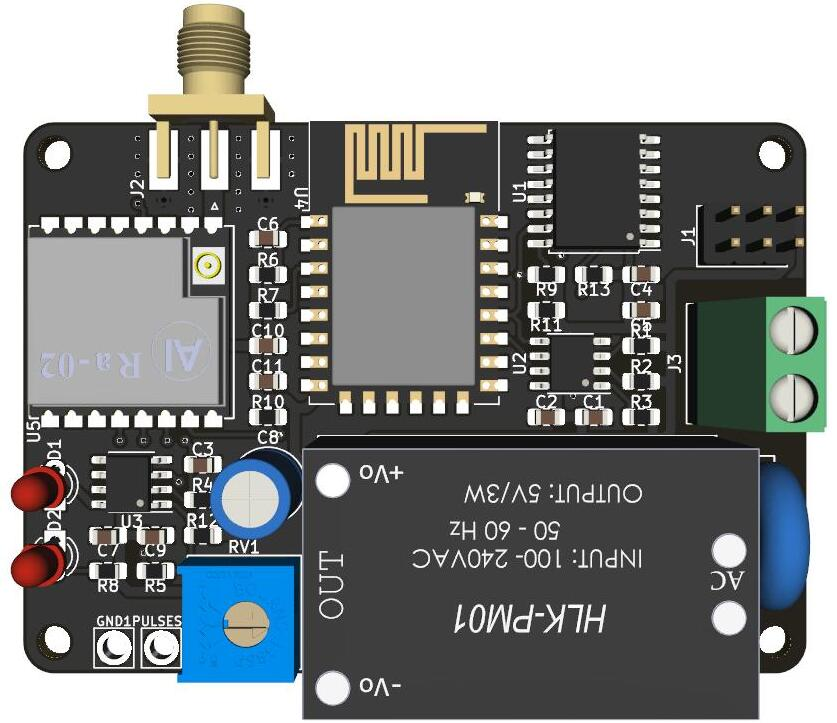
\includegraphics[scale=0.375	]{./Figures/pcb_3d.jpg}
	\caption{Módulo detector de luz.}
		\label{fig:cuadradoAzul}
\end{figure}

La manufactura del PCB fue realizada por el fabricante JLCPCB y los componentes fueron adquiridos de la firma LCSC. Ambos fueron elegidos por los costos reducidos que ofrecen en sus productos, además de que JLCPCB ofrece el servicio de PCBA (\textit{Printed Circuit Board Assembly}, montaje de PCB) con los componentes que tiene disponibles LCSC.